\chapter{The Marriage Feast}

The morning’s sun rose clear and resplendent, touching the foamy waves
into a network of ruby-tinted light.

The feast had been made ready on the second floor at La Réserve, with
whose arbor the reader is already familiar. The apartment destined for
the purpose was spacious and lighted by a number of windows, over each
of which was written in golden letters for some inexplicable reason the
name of one of the principal cities of France; beneath these windows a
wooden balcony extended the entire length of the house. And although
the entertainment was fixed for twelve o’clock, an hour previous to
that time the balcony was filled with impatient and expectant guests,
consisting of the favored part of the crew of the \textit{Pharaon}, and other
personal friends of the bridegroom, the whole of whom had arrayed
themselves in their choicest costumes, in order to do greater honor to
the occasion.

Various rumors were afloat to the effect that the owners of the
\textit{Pharaon} had promised to attend the nuptial feast; but all seemed
unanimous in doubting that an act of such rare and exceeding
condescension could possibly be intended.

Danglars, however, who now made his appearance, accompanied by
Caderousse, effectually confirmed the report, stating that he had
recently conversed with M. Morrel, who had himself assured him of his
intention to dine at La Réserve.

In fact, a moment later M. Morrel appeared and was saluted with an
enthusiastic burst of applause from the crew of the \textit{Pharaon}, who
hailed the visit of the shipowner as a sure indication that the man
whose wedding feast he thus delighted to honor would ere long be first
in command of the ship; and as Dantès was universally beloved on board
his vessel, the sailors put no restraint on their tumultuous joy at
finding that the opinion and choice of their superiors so exactly
coincided with their own.

With the entrance of M. Morrel, Danglars and Caderousse were despatched
in search of the bridegroom to convey to him the intelligence of the
arrival of the important personage whose coming had created such a
lively sensation, and to beseech him to make haste.

Danglars and Caderousse set off upon their errand at full speed; but
ere they had gone many steps they perceived a group advancing towards
them, composed of the betrothed pair, a party of young girls in
attendance on the bride, by whose side walked Dantès’ father; the whole
brought up by Fernand, whose lips wore their usual sinister smile.

Neither Mercédès nor Edmond observed the strange expression of his
countenance; they were so happy that they were conscious only of the
sunshine and the presence of each other.

Having acquitted themselves of their errand, and exchanged a hearty
shake of the hand with Edmond, Danglars and Caderousse took their
places beside Fernand and old Dantès,—the latter of whom attracted
universal notice.

The old man was attired in a suit of glistening watered silk, trimmed
with steel buttons, beautifully cut and polished. His thin but wiry
legs were arrayed in a pair of richly embroidered clocked stockings,
evidently of English manufacture, while from his three-cornered hat
depended a long streaming knot of white and blue ribbons. Thus he came
along, supporting himself on a curiously carved stick, his aged
countenance lit up with happiness, looking for all the world like one
of the aged dandies of 1796, parading the newly opened gardens of the
Luxembourg and Tuileries.

Beside him glided Caderousse, whose desire to partake of the good
things provided for the wedding party had induced him to become
reconciled to the Dantès, father and son, although there still lingered
in his mind a faint and unperfect recollection of the events of the
preceding night; just as the brain retains on waking in the morning the
dim and misty outline of a dream.

\begin{figure}[h]
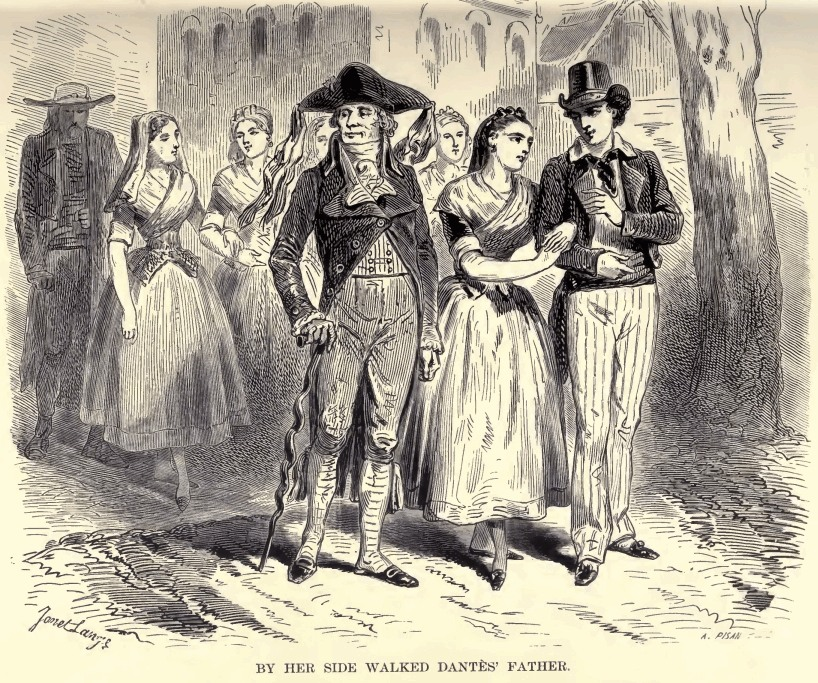
\includegraphics[width=\textwidth]{0065m.jpg}
\end{figure}

As Danglars approached the disappointed lover, he cast on him a look of
deep meaning, while Fernand, as he slowly paced behind the happy pair,
who seemed, in their own unmixed content, to have entirely forgotten
that such a being as himself existed, was pale and abstracted;
occasionally, however, a deep flush would overspread his countenance,
and a nervous contraction distort his features, while, with an agitated
and restless gaze, he would glance in the direction of Marseilles, like
one who either anticipated or foresaw some great and important event.

Dantès himself was simply, but becomingly, clad in the dress peculiar
to the merchant service—a costume somewhat between a military and a
civil garb; and with his fine countenance, radiant with joy and
happiness, a more perfect specimen of manly beauty could scarcely be
imagined.

Lovely as the Greek girls of Cyprus or Chios, Mercédès boasted the same
bright flashing eyes of jet, and ripe, round, coral lips. She moved
with the light, free step of an Arlesienne or an Andalusian. One more
practiced in the arts of great cities would have hid her blushes
beneath a veil, or, at least, have cast down her thickly fringed
lashes, so as to have concealed the liquid lustre of her animated eyes;
but, on the contrary, the delighted girl looked around her with a smile
that seemed to say: “If you are my friends, rejoice with me, for I am
very happy.”

As soon as the bridal party came in sight of La Réserve, M. Morrel
descended and came forth to meet it, followed by the soldiers and
sailors there assembled, to whom he had repeated the promise already
given, that Dantès should be the successor to the late Captain Leclere.
Edmond, at the approach of his patron, respectfully placed the arm of
his affianced bride within that of M. Morrel, who, forthwith conducting
her up the flight of wooden steps leading to the chamber in which the
feast was prepared, was gayly followed by the guests, beneath whose
heavy tread the slight structure creaked and groaned for the space of
several minutes.

“Father,” said Mercédès, stopping when she had reached the centre of
the table, “sit, I pray you, on my right hand; on my left I will place
him who has ever been as a brother to me,” pointing with a soft and
gentle smile to Fernand; but her words and look seemed to inflict the
direst torture on him, for his lips became ghastly pale, and even
beneath the dark hue of his complexion the blood might be seen
retreating as though some sudden pang drove it back to the heart.

During this time, Dantès, at the opposite side of the table, had been
occupied in similarly placing his most honored guests. M. Morrel was
seated at his right hand, Danglars at his left; while, at a sign from
Edmond, the rest of the company ranged themselves as they found it most
agreeable.

Then they began to pass around the dusky, piquant, Arlesian sausages,
and lobsters in their dazzling red cuirasses, prawns of large size and
brilliant color, the echinus with its prickly outside and dainty morsel
within, the clovis, esteemed by the epicures of the South as more than
rivalling the exquisite flavor of the oyster, North. All the
delicacies, in fact, that are cast up by the wash of waters on the
sandy beach, and styled by the grateful fishermen “fruits of the sea.”

“A pretty silence truly!” said the old father of the bridegroom, as he
carried to his lips a glass of wine of the hue and brightness of the
topaz, and which had just been placed before Mercédès herself. “Now,
would anybody think that this room contained a happy, merry party, who
desire nothing better than to laugh and dance the hours away?”

“Ah,” sighed Caderousse, “a man cannot always feel happy because he is
about to be married.”

“The truth is,” replied Dantès, “that I am too happy for noisy mirth;
if that is what you meant by your observation, my worthy friend, you
are right; joy takes a strange effect at times, it seems to oppress us
almost the same as sorrow.”

Danglars looked towards Fernand, whose excitable nature received and
betrayed each fresh impression.

“Why, what ails you?” asked he of Edmond. “Do you fear any approaching
evil? I should say that you were the happiest man alive at this
instant.”

“And that is the very thing that alarms me,” returned Dantès. “Man does
not appear to me to be intended to enjoy felicity so unmixed; happiness
is like the enchanted palaces we read of in our childhood, where
fierce, fiery dragons defend the entrance and approach; and monsters of
all shapes and kinds, requiring to be overcome ere victory is ours. I
own that I am lost in wonder to find myself promoted to an honor of
which I feel myself unworthy—that of being the husband of Mercédès.”

“Nay, nay!” cried Caderousse, smiling, “you have not attained that
honor yet. Mercédès is not yet your wife. Just assume the tone and
manner of a husband, and see how she will remind you that your hour is
not yet come!”

The bride blushed, while Fernand, restless and uneasy, seemed to start
at every fresh sound, and from time to time wiped away the large drops
of perspiration that gathered on his brow.

“Well, never mind that, neighbor Caderousse; it is not worthwhile to
contradict me for such a trifle as that. ’Tis true that Mercédès is not
actually my wife; but,” added he, drawing out his watch, “in an hour
and a half she will be.”

A general exclamation of surprise ran round the table, with the
exception of the elder Dantès, whose laugh displayed the still perfect
beauty of his large white teeth. Mercédès looked pleased and gratified,
while Fernand grasped the handle of his knife with a convulsive clutch.

“In an hour?” inquired Danglars, turning pale. “How is that, my
friend?”

“Why, thus it is,” replied Dantès. “Thanks to the influence of M.
Morrel, to whom, next to my father, I owe every blessing I enjoy, every
difficulty has been removed. We have purchased permission to waive the
usual delay; and at half-past two o’clock the Mayor of Marseilles will
be waiting for us at the city hall. Now, as a quarter-past one has
already struck, I do not consider I have asserted too much in saying,
that, in another hour and thirty minutes Mercédès will have become
Madame Dantès.”

\begin{figure}[h]
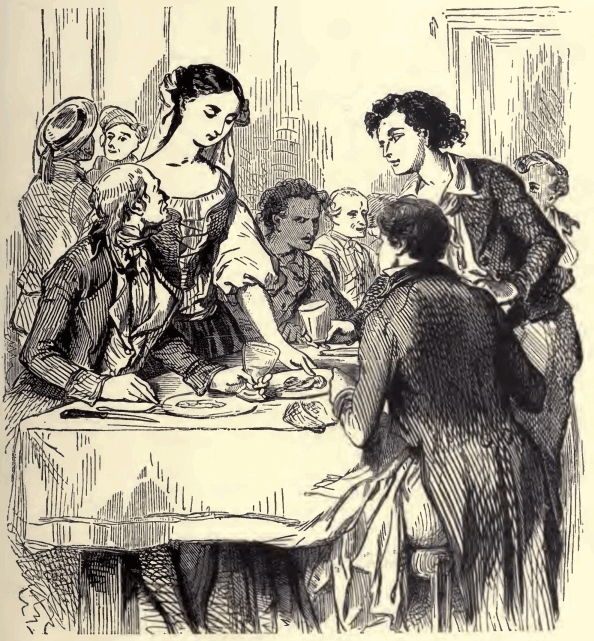
\includegraphics[width=\textwidth]{0069m.jpg}
\end{figure}

Fernand closed his eyes, a burning sensation passed across his brow,
and he was compelled to support himself by the table to prevent his
falling from his chair; but in spite of all his efforts, he could not
refrain from uttering a deep groan, which, however, was lost amid the
noisy felicitations of the company.

“Upon my word,” cried the old man, “you make short work of this kind of
affair. Arrived here only yesterday morning, and married today at three
o’clock! Commend me to a sailor for going the quick way to work!”

“But,” asked Danglars, in a timid tone, “how did you manage about the
other formalities—the contract—the settlement?”

“The contract,” answered Dantès, laughingly, “it didn’t take long to
fix that. Mercédès has no fortune; I have none to settle on her. So,
you see, our papers were quickly written out, and certainly do not come
very expensive.” This joke elicited a fresh burst of applause.

“So that what we presumed to be merely the betrothal feast turns out to
be the actual wedding dinner!” said Danglars.

“No, no,” answered Dantès; “don’t imagine I am going to put you off in
that shabby manner. Tomorrow morning I start for Paris; four days to
go, and the same to return, with one day to discharge the commission
entrusted to me, is all the time I shall be absent. I shall be back
here by the first of March, and on the second I give my real marriage
feast.”

This prospect of fresh festivity redoubled the hilarity of the guests
to such a degree, that the elder Dantès, who, at the commencement of
the repast, had commented upon the silence that prevailed, now found it
difficult, amid the general din of voices, to obtain a moment’s
tranquillity in which to drink to the health and prosperity of the
bride and bridegroom.

Dantès, perceiving the affectionate eagerness of his father, responded
by a look of grateful pleasure; while Mercédès glanced at the clock and
made an expressive gesture to Edmond.

Around the table reigned that noisy hilarity which usually prevails at
such a time among people sufficiently free from the demands of social
position not to feel the trammels of etiquette. Such as at the
commencement of the repast had not been able to seat themselves
according to their inclination rose unceremoniously, and sought out
more agreeable companions. Everybody talked at once, without waiting
for a reply and each one seemed to be contented with expressing his or
her own thoughts.

Fernand’s paleness appeared to have communicated itself to Danglars. As
for Fernand himself, he seemed to be enduring the tortures of the
damned; unable to rest, he was among the first to quit the table, and,
as though seeking to avoid the hilarious mirth that rose in such
deafening sounds, he continued, in utter silence, to pace the farther
end of the salon.

Caderousse approached him just as Danglars, whom Fernand seemed most
anxious to avoid, had joined him in a corner of the room.

“Upon my word,” said Caderousse, from whose mind the friendly treatment
of Dantès, united with the effect of the excellent wine he had partaken
of, had effaced every feeling of envy or jealousy at Dantès’ good
fortune,—“upon my word, Dantès is a downright good fellow, and when I
see him sitting there beside his pretty wife that is so soon to be. I
cannot help thinking it would have been a great pity to have served him
that trick you were planning yesterday.”

“Oh, there was no harm meant,” answered Danglars; “at first I certainly
did feel somewhat uneasy as to what Fernand might be tempted to do; but
when I saw how completely he had mastered his feelings, even so far as
to become one of his rival’s attendants, I knew there was no further
cause for apprehension.” Caderousse looked full at Fernand—he was
ghastly pale.

“Certainly,” continued Danglars, “the sacrifice was no trifling one,
when the beauty of the bride is concerned. Upon my soul, that future
captain of mine is a lucky dog! Gad! I only wish he would let me take
his place.”

“Shall we not set forth?” asked the sweet, silvery voice of Mercédès;
“two o’clock has just struck, and you know we are expected in a quarter
of an hour.”

\begin{figure}[h]
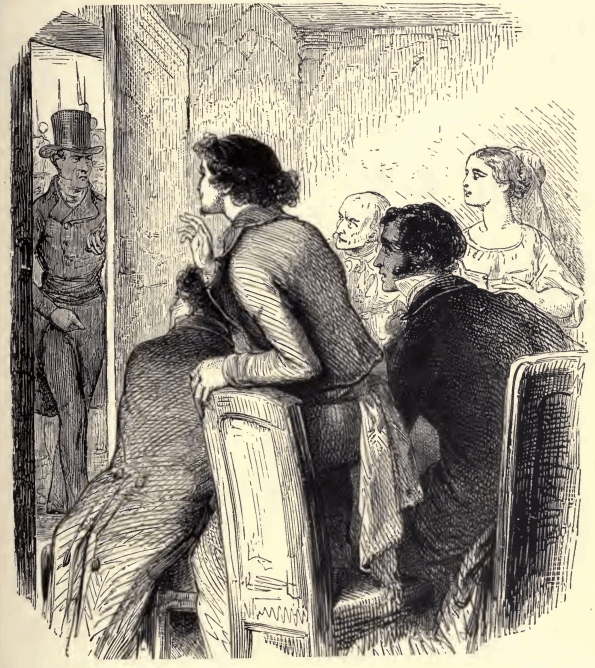
\includegraphics[width=\textwidth]{0071m.jpg}
\end{figure}

“To be sure!—to be sure!” cried Dantès, eagerly quitting the table;
“let us go directly!”

His words were re-echoed by the whole party, with vociferous cheers.

At this moment Danglars, who had been incessantly observing every
change in Fernand’s look and manner, saw him stagger and fall back,
with an almost convulsive spasm, against a seat placed near one of the
open windows. At the same instant his ear caught a sort of indistinct
sound on the stairs, followed by the measured tread of soldiery, with
the clanking of swords and military accoutrements; then came a hum and
buzz as of many voices, so as to deaden even the noisy mirth of the
bridal party, among whom a vague feeling of curiosity and apprehension
quelled every disposition to talk, and almost instantaneously the most
deathlike stillness prevailed.

The sounds drew nearer. Three blows were struck upon the panel of the
door. The company looked at each other in consternation.

“I demand admittance,” said a loud voice outside the room, “in the name
of the law!” As no attempt was made to prevent it, the door was opened,
and a magistrate, wearing his official scarf, presented himself,
followed by four soldiers and a corporal. Uneasiness now yielded to the
most extreme dread on the part of those present.

“May I venture to inquire the reason of this unexpected visit?” said M.
Morrel, addressing the magistrate, whom he evidently knew; “there is
doubtless some mistake easily explained.”

“If it be so,” replied the magistrate, “rely upon every reparation
being made; meanwhile, I am the bearer of an order of arrest, and
although I most reluctantly perform the task assigned me, it must,
nevertheless, be fulfilled. Who among the persons here assembled
answers to the name of Edmond Dantès?”

Every eye was turned towards the young man who, spite of the agitation
he could not but feel, advanced with dignity, and said, in a firm
voice:

“I am he; what is your pleasure with me?”

“Edmond Dantès,” replied the magistrate, “I arrest you in the name of
the law!”

“Me!” repeated Edmond, slightly changing color, “and wherefore, I
pray?”

“I cannot inform you, but you will be duly acquainted with the reasons
that have rendered such a step necessary at the preliminary
examination.”

M. Morrel felt that further resistance or remonstrance was useless. He
saw before him an officer delegated to enforce the law, and perfectly
well knew that it would be as unavailing to seek pity from a magistrate
decked with his official scarf, as to address a petition to some cold
marble effigy. Old Dantès, however, sprang forward. There are
situations which the heart of a father or a mother cannot be made to
understand. He prayed and supplicated in terms so moving, that even the
officer was touched, and, although firm in his duty, he kindly said,
“My worthy friend, let me beg of you to calm your apprehensions. Your
son has probably neglected some prescribed form or attention in
registering his cargo, and it is more than probable he will be set at
liberty directly he has given the information required, whether
touching the health of his crew, or the value of his freight.”

“What is the meaning of all this?” inquired Caderousse, frowningly, of
Danglars, who had assumed an air of utter surprise.

\begin{figure}[h]
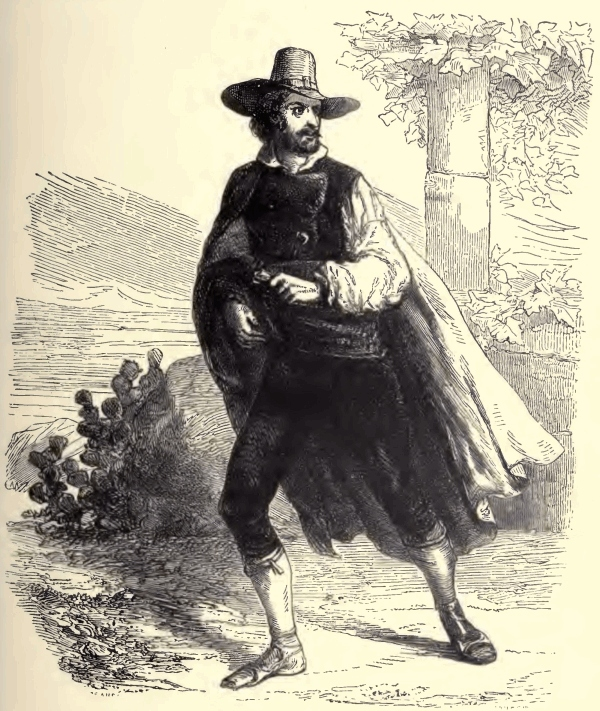
\includegraphics[width=\textwidth]{0073m.jpg}
\end{figure}

“How can I tell you?” replied he; “I am, like yourself, utterly
bewildered at all that is going on, and cannot in the least make out
what it is about.” Caderousse then looked around for Fernand, but he
had disappeared.

The scene of the previous night now came back to his mind with
startling clearness. The painful catastrophe he had just witnessed
appeared effectually to have rent away the veil which the intoxication
of the evening before had raised between himself and his memory.

“So, so,” said he, in a hoarse and choking voice, to Danglars, “this,
then, I suppose, is a part of the trick you were concerting yesterday?
All I can say is, that if it be so, ’tis an ill turn, and well deserves
to bring double evil on those who have projected it.”

“Nonsense,” returned Danglars, “I tell you again I have nothing
whatever to do with it; besides, you know very well that I tore the
paper to pieces.”

“No, you did not!” answered Caderousse, “you merely threw it by—I saw
it lying in a corner.”

“Hold your tongue, you fool!—what should you know about it?—why, you
were drunk!”

“Where is Fernand?” inquired Caderousse.

“How do I know?” replied Danglars; “gone, as every prudent man ought to
be, to look after his own affairs, most likely. Never mind where he is,
let you and I go and see what is to be done for our poor friends.”

During this conversation, Dantès, after having exchanged a cheerful
shake of the hand with all his sympathizing friends, had surrendered
himself to the officer sent to arrest him, merely saying, “Make
yourselves quite easy, my good fellows, there is some little mistake to
clear up, that’s all, depend upon it; and very likely I may not have to
go so far as the prison to effect that.”

\begin{figure}[h]
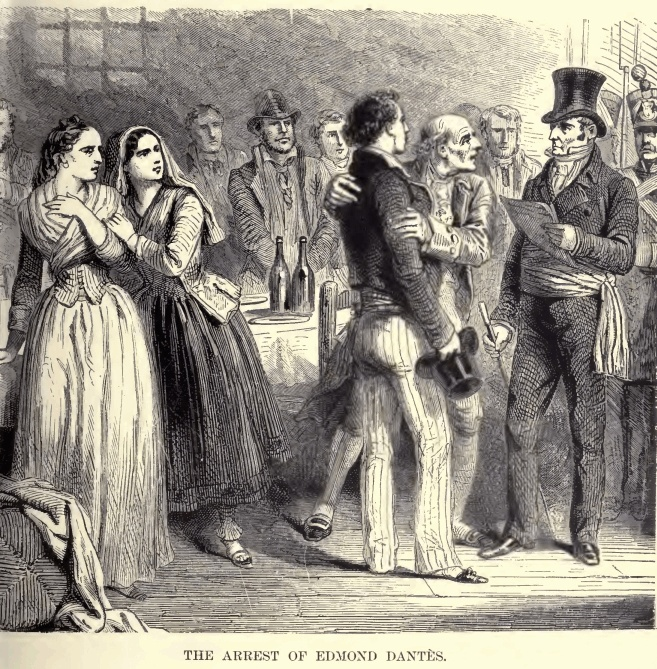
\includegraphics[width=\textwidth]{0075m.jpg}
\end{figure}

“Oh, to be sure!” responded Danglars, who had now approached the group,
“nothing more than a mistake, I feel quite certain.”

Dantès descended the staircase, preceded by the magistrate, and
followed by the soldiers. A carriage awaited him at the door; he got
in, followed by two soldiers and the magistrate, and the vehicle drove
off towards Marseilles.

“Adieu, adieu, dearest Edmond!” cried Mercédès, stretching out her arms
to him from the balcony.

The prisoner heard the cry, which sounded like the sob of a broken
heart, and leaning from the coach he called out, “Good-bye, Mercédès—we
shall soon meet again!” Then the vehicle disappeared round one of the
turnings of Fort Saint Nicholas.

“Wait for me here, all of you!” cried M. Morrel; “I will take the first
conveyance I find, and hurry to Marseilles, whence I will bring you
word how all is going on.”

“That’s right!” exclaimed a multitude of voices, “go, and return as
quickly as you can!”

This second departure was followed by a long and fearful state of
terrified silence on the part of those who were left behind. The old
father and Mercédès remained for some time apart, each absorbed in
grief; but at length the two poor victims of the same blow raised their
eyes, and with a simultaneous burst of feeling rushed into each other’s
arms.

Meanwhile Fernand made his appearance, poured out for himself a glass
of water with a trembling hand; then hastily swallowing it, went to sit
down at the first vacant place, and this was, by mere chance, placed
next to the seat on which poor Mercédès had fallen half fainting, when
released from the warm and affectionate embrace of old Dantès.
Instinctively Fernand drew back his chair.

“He is the cause of all this misery—I am quite sure of it,” whispered
Caderousse, who had never taken his eyes off Fernand, to Danglars.

“I don’t think so,” answered the other; “he’s too stupid to imagine
such a scheme. I only hope the mischief will fall upon the head of
whoever wrought it.”

“You don’t mention those who aided and abetted the deed,” said
Caderousse.

“Surely,” answered Danglars, “one cannot be held responsible for every
chance arrow shot into the air.”

“You can, indeed, when the arrow lights point downward on somebody’s
head.”

Meantime the subject of the arrest was being canvassed in every
different form.

“What think you, Danglars,” said one of the party, turning towards him,
“of this event?”

“Why,” replied he, “I think it just possible Dantès may have been
detected with some trifling article on board ship considered here as
contraband.”

“But how could he have done so without your knowledge, Danglars, since
you are the ship’s supercargo?”

“Why, as for that, I could only know what I was told respecting the
merchandise with which the vessel was laden. I know she was loaded with
cotton, and that she took in her freight at Alexandria from Pastret’s
warehouse, and at Smyrna from Pascal’s; that is all I was obliged to
know, and I beg I may not be asked for any further particulars.”

“Now I recollect,” said the afflicted old father; “my poor boy told me
yesterday he had got a small case of coffee, and another of tobacco for
me!”

“There, you see,” exclaimed Danglars. “Now the mischief is out; depend
upon it the custom-house people went rummaging about the ship in our
absence, and discovered poor Dantès’ hidden treasures.”

Mercédès, however, paid no heed to this explanation of her lover’s
arrest. Her grief, which she had hitherto tried to restrain, now burst
out in a violent fit of hysterical sobbing.

“Come, come,” said the old man, “be comforted, my poor child; there is
still hope!”

“Hope!” repeated Danglars.

“Hope!” faintly murmured Fernand, but the word seemed to die away on
his pale agitated lips, and a convulsive spasm passed over his
countenance.

“Good news! good news!” shouted forth one of the party stationed in the
balcony on the lookout. “Here comes M. Morrel back. No doubt, now, we
shall hear that our friend is released!”

Mercédès and the old man rushed to meet the shipowner and greeted him
at the door. He was very pale.

“What news?” exclaimed a general burst of voices.

“Alas, my friends,” replied M. Morrel, with a mournful shake of his
head, “the thing has assumed a more serious aspect than I expected.”

“Oh, indeed—indeed, sir, he is innocent!” sobbed forth Mercédès.

“That I believe!” answered M. Morrel; “but still he is charged——”

“With what?” inquired the elder Dantès.

“With being an agent of the Bonapartist faction!” Many of our readers
may be able to recollect how formidable such an accusation became in
the period at which our story is dated.

A despairing cry escaped the pale lips of Mercédès; the old man sank
into a chair.

“Ah, Danglars!” whispered Caderousse, “you have deceived me—the trick
you spoke of last night has been played; but I cannot suffer a poor old
man or an innocent girl to die of grief through your fault. I am
determined to tell them all about it.”

“Be silent, you simpleton!” cried Danglars, grasping him by the arm,
“or I will not answer even for your own safety. Who can tell whether
Dantès be innocent or guilty? The vessel did touch at Elba, where he
quitted it, and passed a whole day in the island. Now, should any
letters or other documents of a compromising character be found upon
him, will it not be taken for granted that all who uphold him are his
accomplices?”

With the rapid instinct of selfishness, Caderousse readily perceived
the solidity of this mode of reasoning; he gazed, doubtfully,
wistfully, on Danglars, and then caution supplanted generosity.

“Suppose we wait a while, and see what comes of it,” said he, casting a
bewildered look on his companion.

“To be sure!” answered Danglars. “Let us wait, by all means. If he be
innocent, of course he will be set at liberty; if guilty, why, it is no
use involving ourselves in a conspiracy.”

“Let us go, then. I cannot stay here any longer.”

“With all my heart!” replied Danglars, pleased to find the other so
tractable. “Let us take ourselves out of the way, and leave things for
the present to take their course.”

After their departure, Fernand, who had now again become the friend and
protector of Mercédès, led the girl to her home, while some friends of
Dantès conducted his father, nearly lifeless, to the Allées de Meilhan.

The rumor of Edmond’s arrest as a Bonapartist agent was not slow in
circulating throughout the city.

“Could you ever have credited such a thing, my dear Danglars?” asked M.
Morrel, as, on his return to the port for the purpose of gleaning fresh
tidings of Dantès, from M. de Villefort, the assistant procureur, he
overtook his supercargo and Caderousse. “Could you have believed such a
thing possible?”

“Why, you know I told you,” replied Danglars, “that I considered the
circumstance of his having anchored at the Island of Elba as a very
suspicious circumstance.”

“And did you mention these suspicions to any person beside myself?”

\begin{figure}[h]
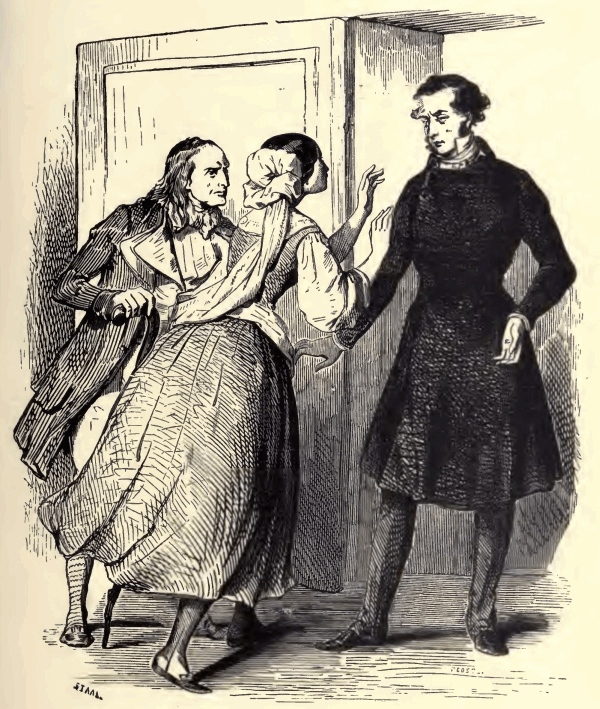
\includegraphics[width=\textwidth]{0079m.jpg}
\end{figure}

“Certainly not!” returned Danglars. Then added in a low whisper, “You
understand that, on account of your uncle, M. Policar Morrel, who
served under the \textit{other} government, and who does not altogether
conceal what he thinks on the subject, you are strongly suspected of
regretting the abdication of Napoleon. I should have feared to injure
both Edmond and yourself, had I divulged my own apprehensions to a
soul. I am too well aware that though a subordinate, like myself, is
bound to acquaint the shipowner with everything that occurs, there are
many things he ought most carefully to conceal from all else.”

“’Tis well, Danglars—’tis well!” replied M. Morrel. “You are a worthy
fellow; and I had already thought of your interests in the event of
poor Edmond having become captain of the \textit{Pharaon}.”

“Is it possible you were so kind?”

“Yes, indeed; I had previously inquired of Dantès what was his opinion
of you, and if he should have any reluctance to continue you in your
post, for somehow I have perceived a sort of coolness between you.”

“And what was his reply?”

“That he certainly did think he had given you offence in an affair
which he merely referred to without entering into particulars, but that
whoever possessed the good opinion and confidence of the ship’s owners
would have his preference also.”

“The hypocrite!” murmured Danglars.

“Poor Dantès!” said Caderousse. “No one can deny his being a
noble-hearted young fellow.”

“But meanwhile,” continued M. Morrel, “here is the \textit{Pharaon} without a
captain.”

“Oh,” replied Danglars, “since we cannot leave this port for the next
three months, let us hope that ere the expiration of that period Dantès
will be set at liberty.”

“No doubt; but in the meantime?”

“I am entirely at your service, M. Morrel,” answered Danglars. “You
know that I am as capable of managing a ship as the most experienced
captain in the service; and it will be so far advantageous to you to
accept my services, that upon Edmond’s release from prison no further
change will be requisite on board the \textit{Pharaon} than for Dantès and
myself each to resume our respective posts.”

“Thanks, Danglars—that will smooth over all difficulties. I fully
authorize you at once to assume the command of the \textit{Pharaon}, and look
carefully to the unloading of her freight. Private misfortunes must
never be allowed to interfere with business.”

“Be easy on that score, M. Morrel; but do you think we shall be
permitted to see our poor Edmond?”

“I will let you know that directly I have seen M. de Villefort, whom I
shall endeavor to interest in Edmond’s favor. I am aware he is a
furious royalist; but, in spite of that, and of his being king’s
attorney, he is a man like ourselves, and I fancy not a bad sort of
one.”

“Perhaps not,” replied Danglars; “but I hear that he is ambitious, and
that’s rather against him.”

“Well, well,” returned M. Morrel, “we shall see. But now hasten on
board, I will join you there ere long.”

So saying, the worthy shipowner quitted the two allies, and proceeded
in the direction of the Palais de Justice.

\begin{figure}[h]
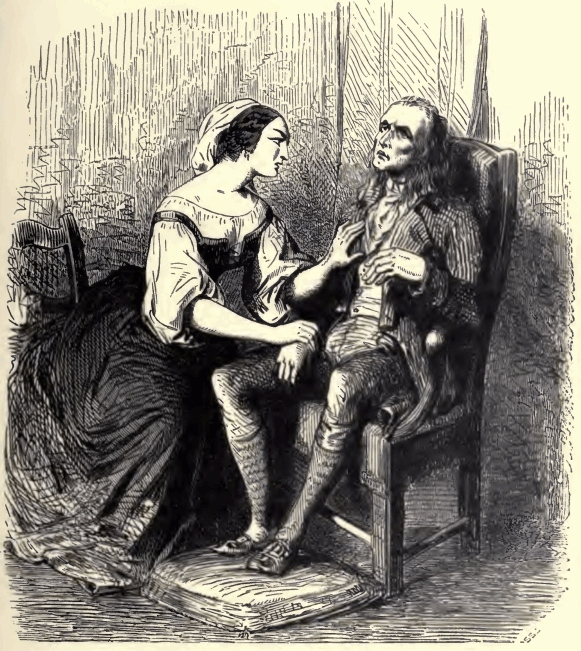
\includegraphics[width=\textwidth]{0081m.jpg}
\end{figure}

“You see,” said Danglars, addressing Caderousse, “the turn things have
taken. Do you still feel any desire to stand up in his defence?”

“Not the slightest, but yet it seems to me a shocking thing that a mere
joke should lead to such consequences.”

“But who perpetrated that joke, let me ask? neither you nor myself, but
Fernand; you knew very well that I threw the paper into a corner of the
room—indeed, I fancied I had destroyed it.”

“Oh, no,” replied Caderousse, “that I can answer for, you did not. I
only wish I could see it now as plainly as I saw it lying all crushed
and crumpled in a corner of the arbor.”

“Well, then, if you did, depend upon it, Fernand picked it up, and
either copied it or caused it to be copied; perhaps, even, he did not
take the trouble of recopying it. And now I think of it, by Heavens, he
may have sent the letter itself! Fortunately, for me, the handwriting
was disguised.”

“Then you were aware of Dantès being engaged in a conspiracy?”

“Not I. As I before said, I thought the whole thing was a joke, nothing
more. It seems, however, that I have unconsciously stumbled upon the
truth.”

“Still,” argued Caderousse, “I would give a great deal if nothing of
the kind had happened; or, at least, that I had had no hand in it. You
will see, Danglars, that it will turn out an unlucky job for both of
us.”

“Nonsense! If any harm come of it, it should fall on the guilty person;
and that, you know, is Fernand. How can we be implicated in any way?
All we have got to do is, to keep our own counsel, and remain perfectly
quiet, not breathing a word to any living soul; and you will see that
the storm will pass away without in the least affecting us.”

“Amen!” responded Caderousse, waving his hand in token of adieu to
Danglars, and bending his steps towards the Allées de Meilhan, moving
his head to and fro, and muttering as he went, after the manner of one
whose mind was overcharged with one absorbing idea.

“So far, then,” said Danglars, mentally, “all has gone as I would have
it. I am, temporarily, commander of the \textit{Pharaon}, with the certainty
of being permanently so, if that fool of a Caderousse can be persuaded
to hold his tongue. My only fear is the chance of Dantès being
released. But, there, he is in the hands of Justice; and,” added he
with a smile, “she will take her own.” So saying, he leaped into a
boat, desiring to be rowed on board the \textit{Pharaon}, where M. Morrel had
agreed to meet him.
